%! Author = adnansiddiquei
%! Date = 19/03/2024

\section{Training the model}\label{sec:q1bc}
\begin{figure}[t]
    \centering
    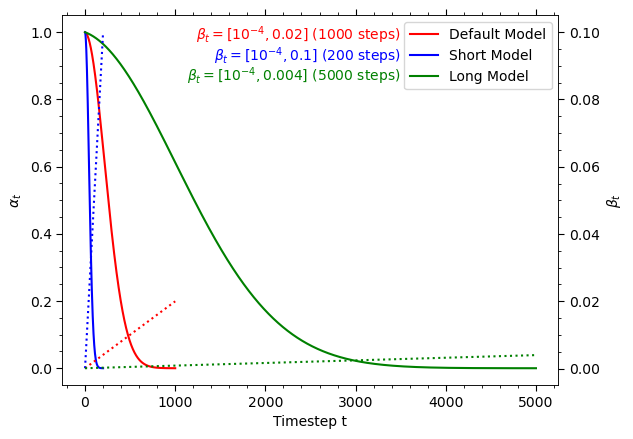
\includegraphics[width=0.8\textwidth]{figures/q1b_noise_schedules}
    \caption{A plot of each noise schedule that was evaluated.
        The dotted lines represent the $\beta_{t}$ values and the solid lines represent the $\alpha_t$ values.}
    \label{fig:q1b_noise_schedules}
\end{figure}

\begin{figure}[t]
    \centering
    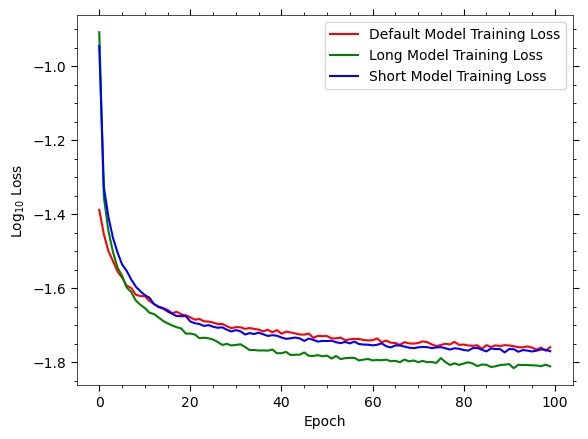
\includegraphics[width=0.8\textwidth]{figures/q1b_training_loss}
    \caption{A plot of the training loss for each model over 100 epochs.}
    \label{fig:q1b_training_loss}
\end{figure}

\begin{figure}
\centering
\begin{subfigure}{0.8\textwidth}
    \centering
    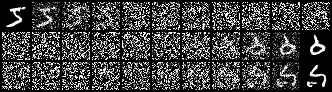
\includegraphics[width=1\textwidth]{./figures/q1b_def_model_nd}
    \caption{The encoding and decoding process for the default model, with each column representing equal time steps
        apart (100 time steps).}
    \label{fig:q1b_def_model_nd}
\end{subfigure}%
\hfill
\begin{subfigure}{0.8\textwidth}
    \centering
    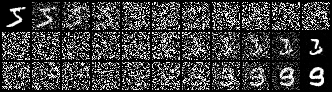
\includegraphics[width=1\textwidth]{./figures/q1b_short_model_nd}
    \caption{The encoding and decoding process for the short model, with each column representing equal time steps
        apart (20 time steps).}
    \label{fig:q1b_short_model_nd}
\end{subfigure}
\hfill
\begin{subfigure}{0.8\textwidth}
    \centering
    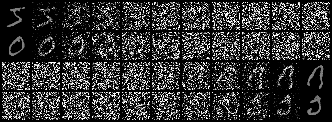
\includegraphics[width=1\textwidth]{./figures/q1b_long_model_nd}
    \caption{The encoding and decoding process for the long model, with each column representing equal time steps
        apart (500 time steps).}
    \label{fig:q1b_long_model_nd}
\end{subfigure}
\caption{The encoding and decoding process for each of the models trained in Section~\eqref{sec:q1bc}.}
\label{fig:q1b_short_long_model_nd}
\end{figure}

\begin{figure}
\centering
\begin{subfigure}{0.8\textwidth}
    \centering
    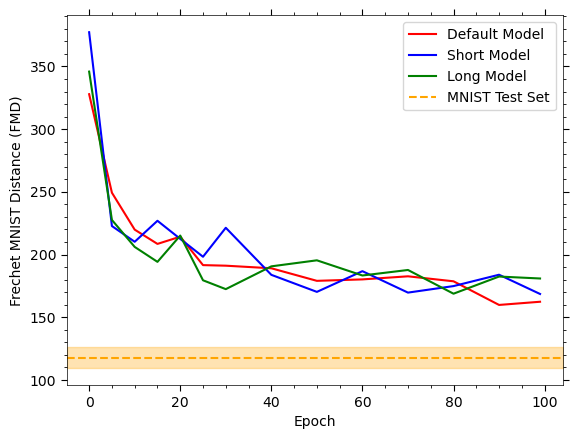
\includegraphics[width=0.85\textwidth]{figures/q1b_fmd}
    \caption{The raw FMD values for each model, with the orange line showing mean and standard deviation of
        the FMD value for 15 random samples from the MNIST test set.}
    \label{fig:q1b_fmd_not_norm}
\end{subfigure}%
\hfill
\begin{subfigure}{0.8\textwidth}
    \centering
    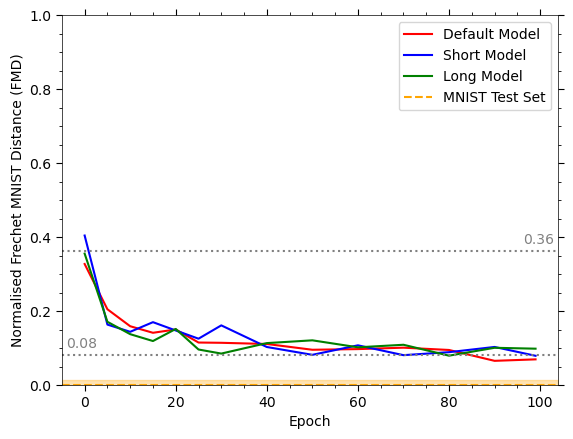
\includegraphics[width=0.85\textwidth]{./figures/q1b_fmd_normalised}
    \caption{The same FMD values as above, but normalised between 0 and 1, where 0 is the mean FMD value for the MNIST
        test set (as shown on the above figure) and 1 is the FMD value for a completely black image.
        The grey dotted lines show the mean start and end values.}
    \label{fig:q1b_fmd_normalised}
\end{subfigure}
\caption{Two plots of the Frechet MNIST Distance (FMD) for the generated samples from each model over 100 epochs.
        The top plot is normalised, the bottom is not.
        At each plotted epoch, 32 samples were generated from the model and compared against the first 512 samples from the
        MNIST test dataset.}
\label{fig:q1b_fmd}
\end{figure}

\begin{figure}
\centering
\begin{subfigure}{0.8\textwidth}
    \centering
    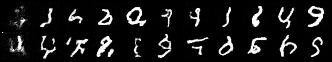
\includegraphics[width=1\textwidth]{figures/q1b_samples_def}
    \caption{The default model.}
    \label{fig:q1b_samples_def}
\end{subfigure}%
\hfill
\begin{subfigure}{0.8\textwidth}
    \centering
    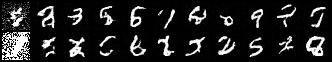
\includegraphics[width=1\textwidth]{./figures/q1b_samples_short}
    \caption{The short model.}
    \label{fig:q1b_samples_short}
\end{subfigure}
\hfill
\begin{subfigure}{0.8\textwidth}
    \centering
    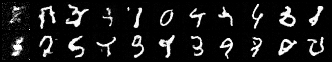
\includegraphics[width=1\textwidth]{./figures/q1b_samples_long}
    \caption{The long model.}
    \label{fig:q1b_samples_long}
\end{subfigure}
\caption{The samples generated by each model at every 10 epochs. Epoch 1 is on the left, and epoch 100 is on the right.}
\label{fig:q1b_samples}
\end{figure}

\begin{figure}
\centering
\begin{subfigure}{0.3\textwidth}
    \centering
    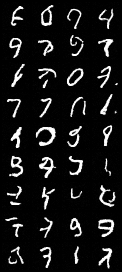
\includegraphics[width=1\textwidth]{figures/q1b_samples_def_final}
    \caption{The default model.}
    \label{fig:q1b_samples_def_final}
\end{subfigure}%
\hfill
\begin{subfigure}{0.3\textwidth}
    \centering
    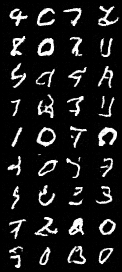
\includegraphics[width=1\textwidth]{./figures/q1b_samples_short_final}
    \caption{The short model.}
    \label{fig:q1b_samples_short_final}
\end{subfigure}
\hfill
\begin{subfigure}{0.3\textwidth}
    \centering
    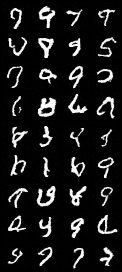
\includegraphics[width=1\textwidth]{./figures/q1b_samples_long_final}
    \caption{The long model.}
    \label{fig:q1b_samples_long_final}
\end{subfigure}
\caption{36 samples generated by each model at the final epoch.}
\label{fig:q1b_samples_final}
\end{figure}

This section discusses the training of the DDPM model with varying linear noise schedules.

Three different models were trained, the first model (default model) was trained with the provided noise schedule:
$\beta_{t} = [10^{-4}, 0.02]$ with 1000 steps; the second model (the "long model") was trained with a longer noise schedule:
$\beta_{t} = [10^{-4}, 0.004]$ with 5000 steps which added less noise at each step; and the third model (the "short model")
was trained with a shorter noise schedule: $\beta_{t} = [10^{-4}, 0.1]$ with 200 steps which added more noise at each step.
The number of steps was amended for each model such that the final noise level was the same for each model ($\alpha_{t}$
of the order of $10^{-5}$ at the final time step).
All models were also trained for 100 epochs with a batch size of 128, with the Adams optimiser, a learning rate of
$2 \times 10^{-4}$.
The CNN architecture for all models was identical to as described in Section~\eqref{sec:q1a}, with exception
that the number of \inlinecode{CNNBlocks} was increased by 1 (from $[16, 32, 32, 16, 1]$ to $[16, 32, 64, 32, 16, 1]$ where
the numbers indicate the number of channels in each layer).
This was increased whilst considering the trade-off between fidelity of the generated samples and the computational cost of training.
Additionally, the \inlinecode{transforms.Normalize((0.5,), (1.0))} step was removed from the MNIST dataset transformation
to allow for more equivocal comparison between the these models and the custom degradation model implemented in Section~\eqref{sec:q2}
(more on this later).

Figure~\eqref{fig:q1b_noise_schedules} illustrates the noise schedules used for each model, Figure~\eqref{fig:q1b_training_loss}
shows the training loss for each model over 100 epochs, and Figure~\eqref{fig:q1b_short_long_model_nd} illustrates the encoding
and decoding process for all 3 models.
Figure~\eqref{fig:q1b_fmd} shows the Frechet MNIST Distance (FMD) for the generated samples from each model as the model
is trained over the 100 epochs.
The FMD is an adjusted version of the Frechet Inception Distance (FID) which uses an MNIST classifier (that was trained
for this purpose) with a 1024-length feature vector at the penultimate layer to calculate the Frechet distance instead
of the InceptionV3 model.
See Appendix~\eqref{app:mnist-classifier} for more details on the MNIST classifier that was used to calculate the FMD.
The FMD was used instead of the FID as the MNIST dataset is a narrow context dataset and so a model trained specifically on this
dataset would be more appropriate for calculating the Frechet distance.

From these figures, several conclusions can be drawn.
All models show convergence in their training loss and converge to similar values, with very little instability in the training.
The FMD score falls in a correlated fashion to the training loss, indicating that the models are indeed generating samples
that are statistically similar to the MNIST dataset.
However, neither model outperforms the others by any significant means across either of these metrics.
Figure~\eqref{fig:q1b_fmd_normalised} indicates a 4.5x mean decrease in the FMD values, however on inspection to
Figure~\eqref{fig:q1b_samples} and Figure~\eqref{fig:q1b_samples_final}, the samples generated by these models are still
fairly poor, and so a normalised FMD value of 0.08 is still not particularly impressive.
